\chapter{The Large Hadron Collider and the \ATLAS Detector}\label{chap:lhc_atlas}

%AB: The work presented in this thesis relies on data recorded by the ATLAS detector in high energy proton-proton collisions. This chapter provides an overview of the experimental apparatus and analysis techniques used throughout this thesis.

The Large Hadron Collider (\LHC) at \CERN has extended the frontiers of particle physics through its unprecedented energy and luminosity.
The \LHC accelerates protons around a \SI{27}{\km} ring until they are travelling just \SI{3}{\m\per\s} slower than than the speed of light, at which point they are made to collide.
The protons travel round the ring 11 thousand times per second in two concentric beams, which are guided by superconducting magnets cooled using liquid helium to \SI{-271.3}{\degreeCelsius} (\SI{1.9}{\kelvin}).
The beams travel in opposite directions and are crossed at four locations so that collisisons between protons can take place.
Around these collision points four specialised detectors, ALICE~\cite{AliceCollaboration_2008}, CMS~\cite{CMS-TDR-08-001}, LHCb~\cite{LHCbCollaboration_2008} and \ATLAS~\cite{PERF-2007-01}, are located to capture information about the products of the collisions.

\begin{comment}
  An overview of the LHC complex is presented in Figure 3.1. Hydrogen gas is ionised using an
  electric field. The first accelerator in the chain, Linac 2, accelerates these protons to 50 MeV. The
  Proton Synchrotron Booster then accelerates the protons to 1.4 GeV, before they are accelerated to
  25 GeV by the Proton Synchrotron. The energy of the beam is further increased to 450 GeV by the
  Super Proton Synchrotron, before it is split into the two beampipes of the LHC. At this final stage,
  the beams are accelerated to an energy of 6.5 TeV (for Run-2) [25, 27]. Proton bunches are spaced
  by 25 ns, with each bunch containing up to 1.1 × 1011 protons.
\end{comment}

The \LHC is operated in \textit{runs} during which beams of protons are actively being circulated and collided. Between runs which there are periods of shutdown while the accelerator and detector machinery is maintained and upgraded.
In 2010, the \LHC collided proton bunches, each containing more than $10^{11}$ particles, 20 million times per second, providing \SI{7}{\TeV} proton-proton collisions at instantaneous luminosities of up to \peakLumi.
\runtwo, which began in 2015, increased the the proton-proton collision energy to \SI{13}{\TeV}.
The bunch spacing was also reduced, leading to a collisison rate of \SI{40}{\mega\hertz}.
Over the course of \runtwo a total integrated luminosity of \runtwointlumi was recorded. % less good for physics
2022 marked the beginning of \runthree which, with a higher center of mass energy and peak luminosity, is expected to culminate in the approximate doubling of the dataset size.
%We will be focusing the proton beams at the interaction points to less than 10 micron beam size, to increase the collision rate. (nominal beam size (width) is 16 microns from around run1)

\begin{table}[!htbp]
  \footnotesize\centering
  \setlength{\tabcolsep}{0.5em} % for the horizontal padding
  \begin{tabular}{cc|cccc}
      \toprule 
      \textbf{Period} & \textbf{Year} & $\sqrt{s}$ [\unit\TeV] 
      & \angles{\mu} & \textbf{Bunch spacing} [\unit\ns] & \textbf{Luminosity} [\unit\invcmsqpersec] \\
      \hline
      Run 1 & 2011--2012 & \SIrange[range-phrase=--,range-units=single,range-exponents=combine]{7}{8}{} & 18 & 50 & $8 \times 10^{33}$ \\
      Run 2 & 2015--2018 & \SI{13  }{} & 34 & 25 & $1\textnormal{--}2 \times 10^{34}$ \\
      Run 3 & 2022--2025 & \SI{13.6}{} & 50 & 25 & $2 \times 10^{34}$ \\
      \bottomrule
  \end{tabular}
  \caption{
    Overview of the different LHC runs \cite{atlas-lumi-run1,atlas-lumi-run2}.
    The average number of interactions per bunch-crossing is denoted as \angles{\mu} (see \cref{sec:collider_defs}).
    Numbers for Run 3 are preliminary and are only provided to give an indication of expected performance.
    % run 1 run 2 trigger https://cds.cern.ch/record/2058218/
    %  2-3 × 1034 cm−2 s−1 and an average pile-up of ~80 collisions/bunch-crossing
    % https://cds.cern.ch/record/2732959/files/LHCP2020_094.pdf
  }
  \label{tab:lhc_runs}
\end{table}


\section{Coordinate System \& Collider Definitions}

\subsection{ATLAS Coordinate System}

%% from https://twiki.cern.ch/twiki/bin/view/AtlasProtected/PubComCommonText
% ATLAS coordinate system
ATLAS uses a right-handed coordinate system with its origin at the nominal interaction point in the centre of the detector and the \axis{z} along the beam pipe. The \axis{x} points from the interaction point to the centre of the LHC ring, and the \axis{y} points upwards. Cylindrical coordinates \((r,\phi)\) are used in the transverse plane, \(\phi\) being the azimuthal angle around the \axis{z}. The pseudorapidity is defined in terms of the polar angle \(\theta\) as \(\eta = -\ln \tan(\theta/2)\). Angular distance is measured in units of \(\DeltaR \equiv \sqrt{(\Delta\eta)^{2} + (\Delta\phi)^{2}}\).\todo{this is from pubcom}

The transverse plane lies in $x$\nobreakdash-$y$ while the longitudinal plane lies along the \axis{z}.
%
\begin{figure}[!htbp]
  \centering
  % Author: Izaak Neutelings (June 2017)
% taken from https://tex.stackexchange.com/questions/159445/draw-in-cylindrical-and-spherical-coordinates
% Licensed under CC Attribution-Share Alike 4.0 International  https://creativecommons.org/licenses/by-sa/4.0/
% Original source https://wiki.physik.uzh.ch/cms/latex:example_spherical_coordinates
% Modifications by Giles Strong (March 2020):
% 1. Removal of some header code
% 2. Changing theta to eta
% 3. Addition of mountains
% 4. Changed "\draw[dashed,red] (O)  -- (Pxy);" to "\draw[->] (O)  -- (Pxy) node[right] {$p_t$};"
% Modifications by Giles Strong (April 2020):
% 1. Removal of Jura mountains
% 2. Rotated to be in terms of ATLAS coordinate system
% 3. Resized labels for the detectors

\tikzset{>=latex} % for LaTeX arrow head

\tdplotsetmaincoords{75}{50} % to reset previous setting 75 50
    \begin{tikzpicture}[scale=2.7,tdplot_main_coords,rotate around x=90]
    
    % variables
    \def\rvec{1.2}
    \def\thetavec{40}
    \def\phivec{70}
    \def\R{1.1}
    \def\w{0.3}
    
    % axes
    \coordinate (O) at (0,0,0);
    \draw[thick,->] (0,0,0) -- (1,0,0) node[below left]{$x$};
    \draw[thick,->] (0,0,0) -- (0,1,0) node[below right]{$y$};
    \draw[thick,->] (0,0,0) -- (0,0,1) node[below right]{$z$};
    \tdplotsetcoord{P}{\rvec}{\thetavec}{\phivec}
    
    % vectors
    \draw[->,red] (O) -- (P) node[above left] {$\overrightarrow{p}$};
    \draw[->] (O)  -- (Pxy) node[right] {$p_t$};
    \draw[dashed,red] (P)  -- (Pxy);
    \draw[dashed,red] (Py) -- (Pxy);
    
    % circle - LHC
    \tdplotdrawarc[thick,rotate around x=90,black!70!blue]{(\R,0,0)}{\R}{0}{360}{}{}
    
    % compass - the line between CMS and ATLAS has a ~12° declination (http://googlecompass.com)
    \begin{scope}[shift={(1.1*\R,0,1.65*\R)},rotate around y=12]
        \draw[<->,black!50] (-\w,0,0) -- (\w,0,0);
        \draw[<->,black!50] (0,0,-\w) -- (0,0,\w);
        \node[below right,black!50,scale=0.6] at (\w,0,0) {N};
    \end{scope}
    
    % nodes
    \node[right] at (\R,0,0) {LHC};
    \fill[radius=0.8pt,black!20!red]
        (O) circle node[left=4pt,below=5pt] {ATLAS};
    \draw[thick] (0.02,0,0) -- (0.5,0,0); % partially overdraw x-axis and CMS point
    \fill[radius=0.8pt,black!20!blue]
        (2*\R,0,0) circle
        node[right=4pt,below=2pt,scale=0.7] {CMS};
    \fill[radius=0.8pt,black!10!orange]
        ({-\R*sqrt(2)/2+\R},0,{-\R*sqrt(2)/2}) circle % 45 degrees from ATLAS
        node[left=2pt,below=2pt,scale=0.7] {ALICE};
    \fill[radius=0.8pt,black!60!green]
        ({-\R*sqrt(2)/2+\R},0,{\R*sqrt(2)/2}) circle % 45 degrees from ATLAS
        node[below=6pt,right=3pt,scale=0.7,anchor=north east] {LHCb};
    
    % arcs
    \tdplotdrawarc[->]{(O)}{0.2}{0}{\phivec}
        {above=2pt,right=-1pt,anchor=mid west}{$\phi$}
    \tdplotdrawarc[->,rotate around z=\phivec-90,rotate around y=-90]{(0,0,0)}{0.5}{0}{\thetavec}
        {anchor=mid east}{$\eta$}
\end{tikzpicture}
  \caption{
    The coordinate system used at the ATLAS detector, showing the locations of the four main experiments located at various points around the LHC.
    Reproduced from \rcite{Strong:2020mge}.
  }
  \label{fig:atlas_coord_system}
\end{figure}

The polar angle $\theta$ is commonly specified in terms of the pseudorapidity $\eta$, defined as
%
\begin{equation}\label{eq:pseudorap}
  \eta = - \ln \left[ \tan \left( \frac{\theta}{2} \right) \right] .
\end{equation}
%
Differences in $\eta$ are invariant under Lorentz boosts. Particle production is constant as a function of $\eta$.
%particle production is constant as a function of rapidity, and because differences in rapidity are Lorentz invariant under boosts along the longitudinal axis: they transform additively, similar to velocities in Galilean relativity. A

The transverse momentum \pt is the sum in quadrature of the momenta in the transverse plane
%
\begin{equation}\label{eq:pt}
  \pt = \sqrt{ {p_x}^2 + {p_y}^2 } .
\end{equation}

Transverse and longitudinal impact pararameters (IP) \dzero and \zzero specify the closest approach of the trajectory of a particle to the origin.
The transverse IP \dzero and longitudinal IP \zzero are measured with respect to the hard scatter primary vertex (see \cref{sec:vertex_reco}).

%\textbf{Lorentz angle}. The Lorentz angle $\theta_L$ is the angle between the electric field and the direction of the drift of the electron and holes in a silicon strip or pixel detector, when submerged in a magnetic field.


\subsection{Collider Definitions}\label{sec:collider_defs}

\subsubsection{Luminosity}
The luminosity is defined by\todo{xy full def}
%
\begin{equation}\label{eq:lumi_def}
L = \frac{1}{\sigma} \der{N}{t} = \frac{f n_b N_1 N_2}{2 \pi \sigma_x \sigma_y},
\end{equation}
%
where $N$ is the number of individual proton-proton collisions and $\sigma$ is the cross-sectional area of the beams as they cross.

Total number of events is related to the total inelastic cross section\todo{define}
%
\begin{equation}
 N = \sigma \int \mathcal{L} ~\mathrm{d}t 
\end{equation}
%

%
\begin{figure}[!htbp]
  \centering
  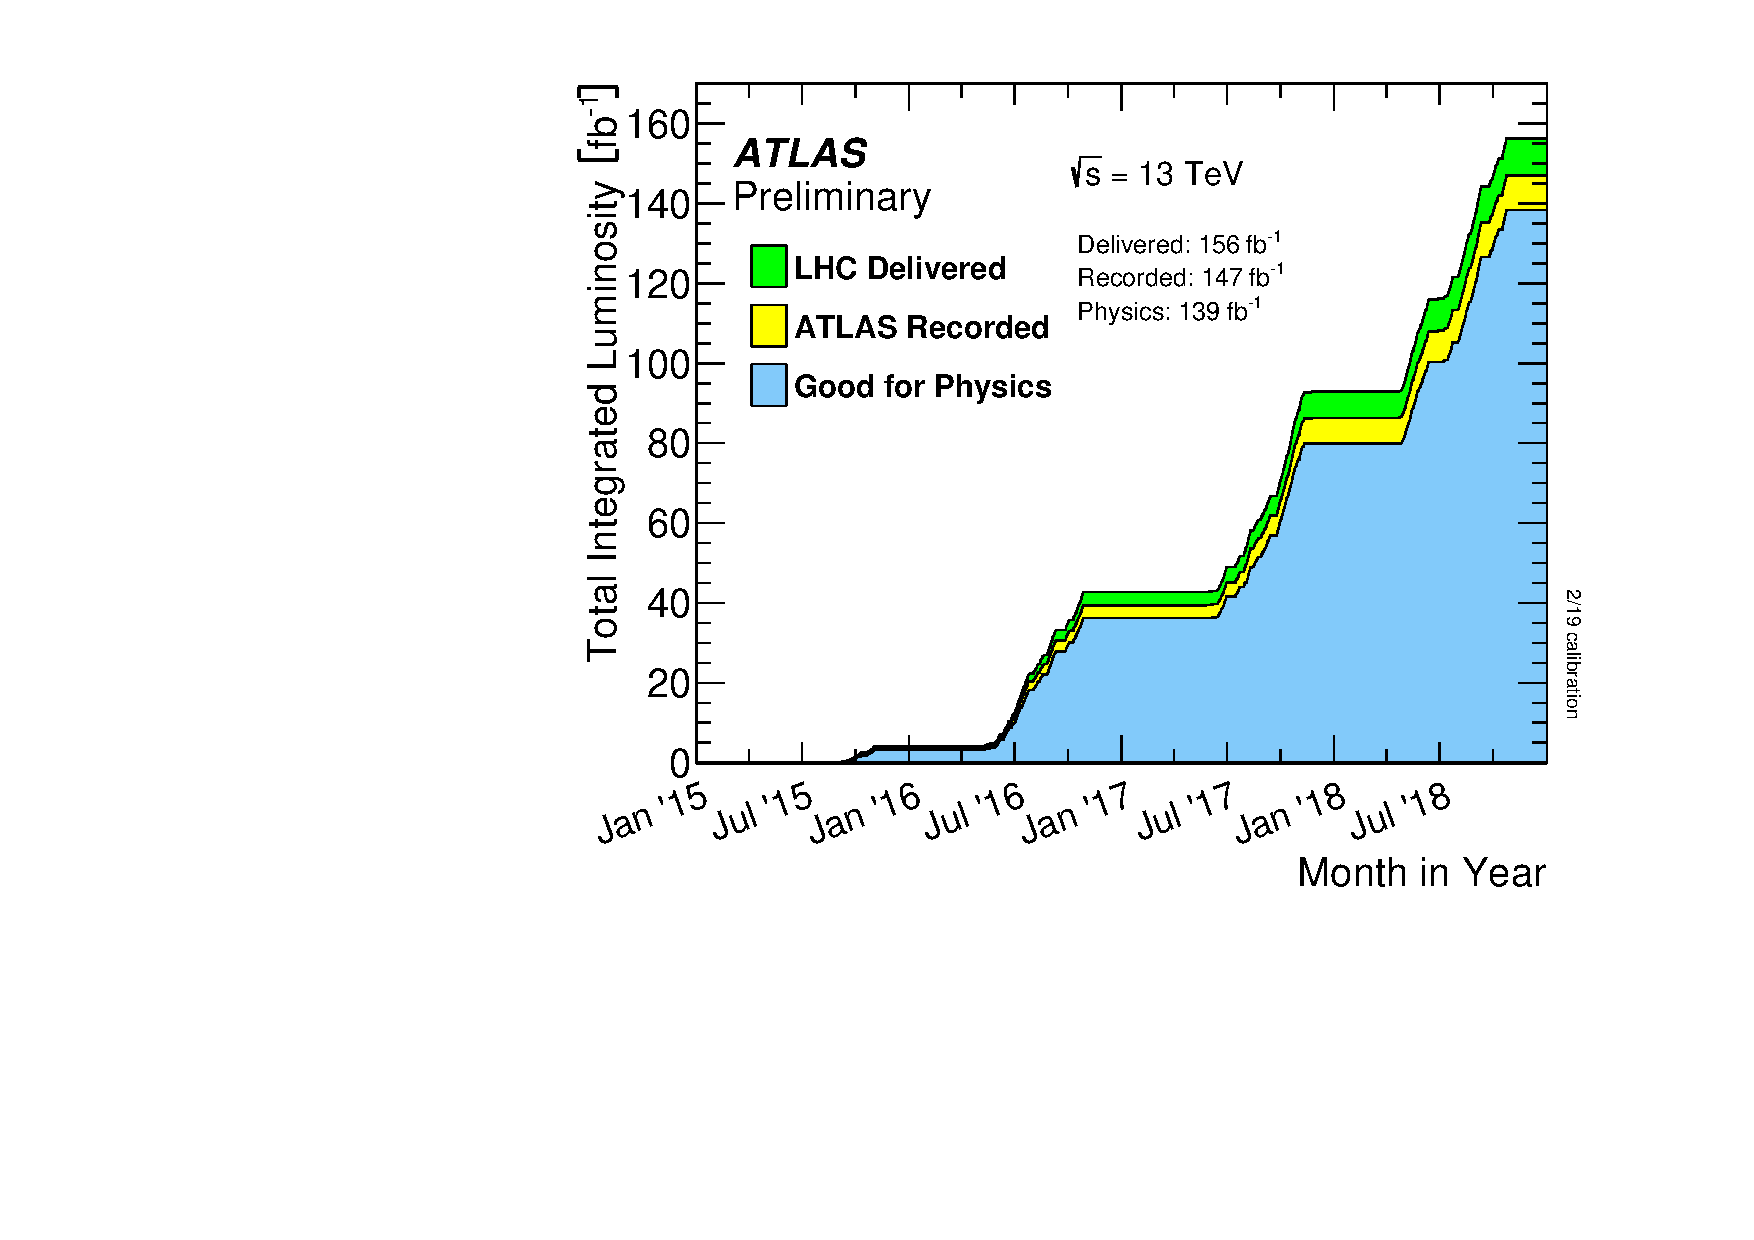
\includegraphics[width=0.6\linewidth]{chapters/2.detector/figs/intlumivstimeRun2DQall.pdf}
  \caption{
    Delivered, recorded, and usable integrated luminosity as a function of time during \runtwo \cite{atlas-lumi-run2}.
  }
  \label{fig:run2_lumi}
\end{figure}
%


\subsubsection{Pile-up}

At the centre of the ATLAS detector, bunches of more than $10^{11}$ protons meet head on.
Each bunch-crossing is called an \textit{event}.
There is generally at most one hard proton-proton scatter per event.
Additional interactions are typically relatively soft and are known as \textit{pile-up}.
Pile-up complicates the reconstruction of the hard scatter event as results of the interactions of different proton-proton interactions have to be separated.
Pile-up from interactions within the same bunch-crossing is known as \textit{in-time} pile-up while residual signatures from other bunch-crossings is known as \textit{out-of-time} pile-up.
The number of pile-up interactions is denoted $\mu$, which is often given as a time-averaged value \angles{\mu}.
The average number of pile-up interactions for different years during \runtwo is given in \cref{fig:run2_pile-up}.
%
\begin{figure}[!htbp]
  \centering
  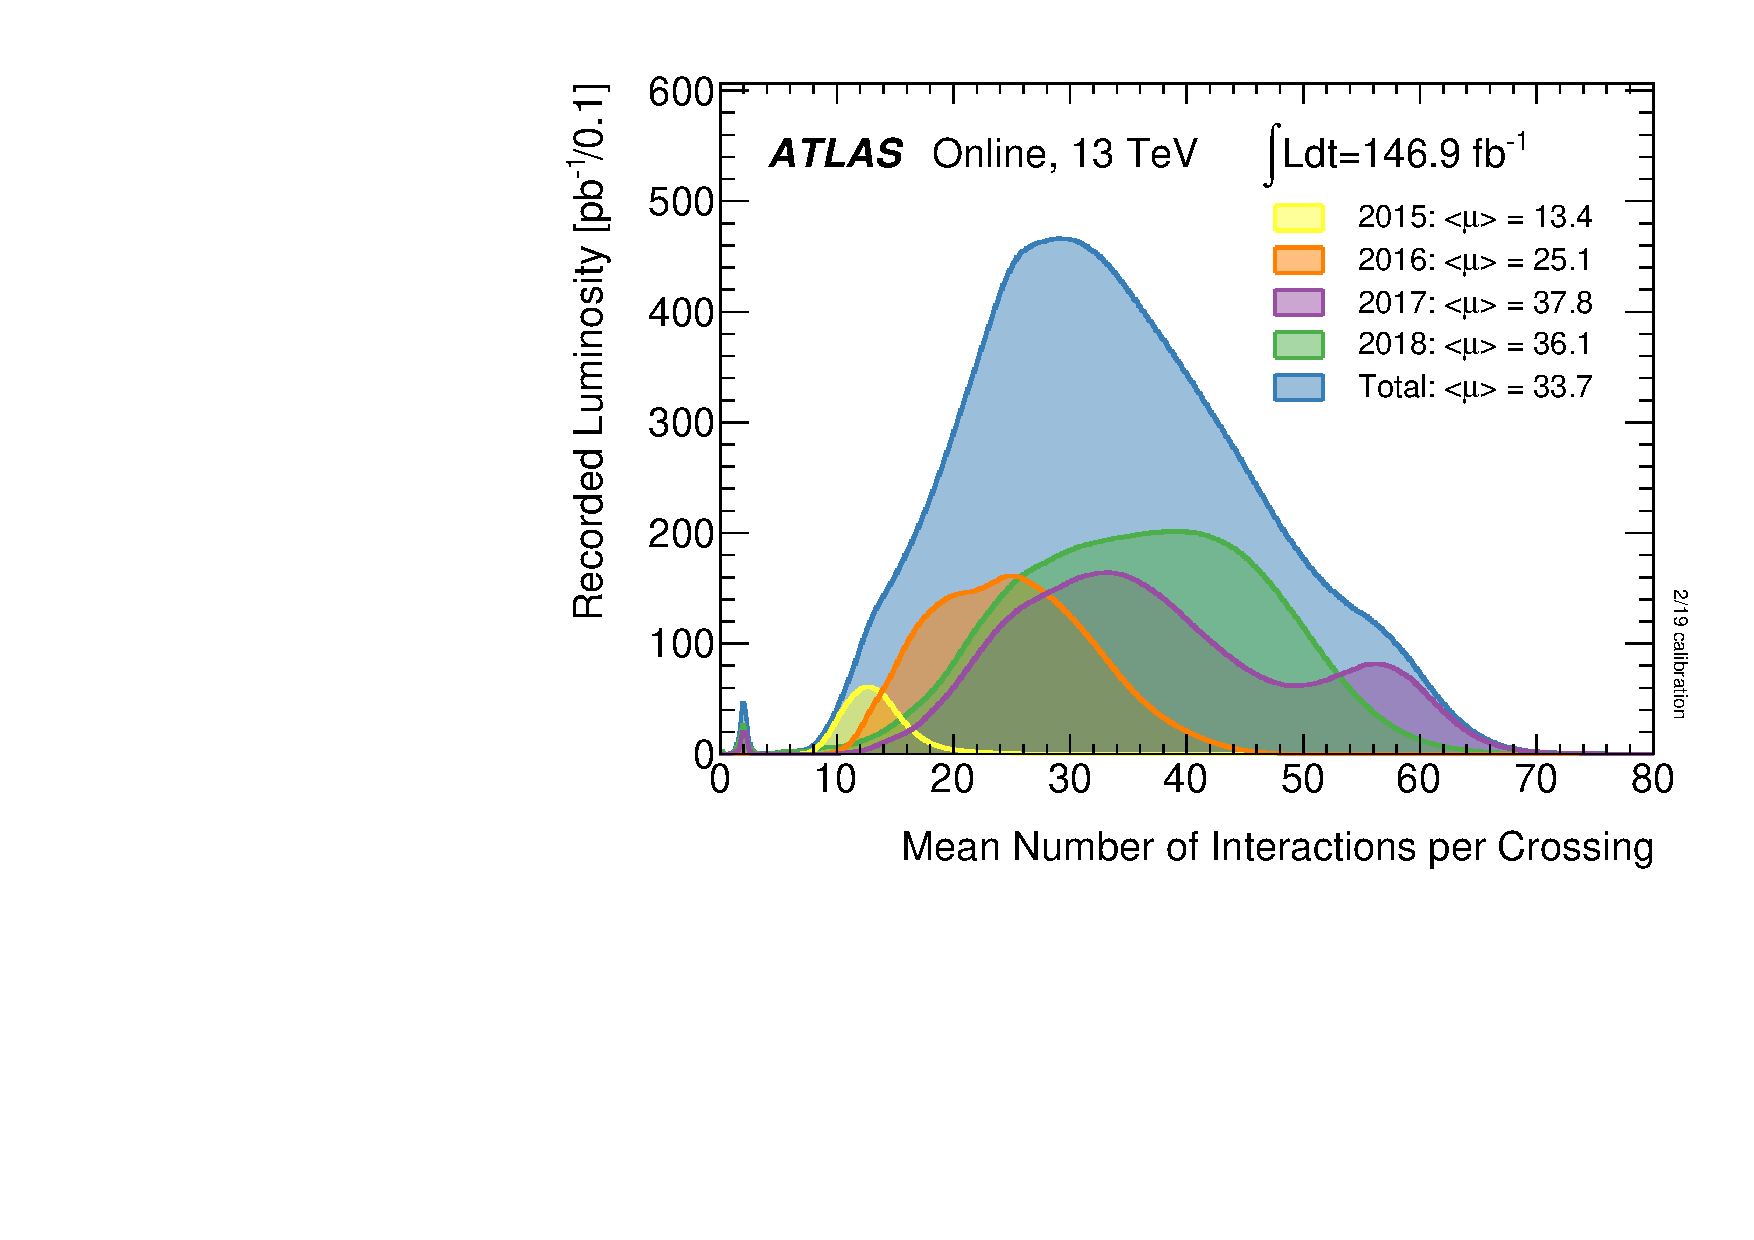
\includegraphics[width=0.6\linewidth]{chapters/2.detector/figs/mu_2015_2018.pdf}
  \caption{
    Average pile-up profiles measured by ATLAS during \runtwo \cite{atlas-lumi-run2}.
    During \runthree, even higher levels of pile-up are expected.
  }
  \label{fig:run2_pile-up}
\end{figure}
%


\section{The ATLAS Detector}\label{sec:atlas_detector}
\todo{suggestion: make the first sentence more of a inutitive understanding, and then go into barel eta encap jargon}

The ATLAS\footnote{A Toroidal Lhc ApparatuS.} detector at the LHC covers nearly the entire solid angle around the collision point.
It consists of an inner tracking detector surrounded by a thin superconducting solenoid, electromagnetic and hadronic calorimeters,
and a muon spectrometer incorporating three large superconducting air-core toroidal magnets.\todo{okay this is the standard pubcom text?}

The detector is made up of several specialised sub-detectors as shown in \cref{fig:atlas_detector}.
In this section a condensed overview of each sub-detector is given, in order of increasing radial distance from the point of collision.
A more complete picture can be found in \rcite{PERF-2007-01}, or in the technical design reports (TDRs) of the individual sub-detectors.

\begin{figure}[!htpb]
  \centering
  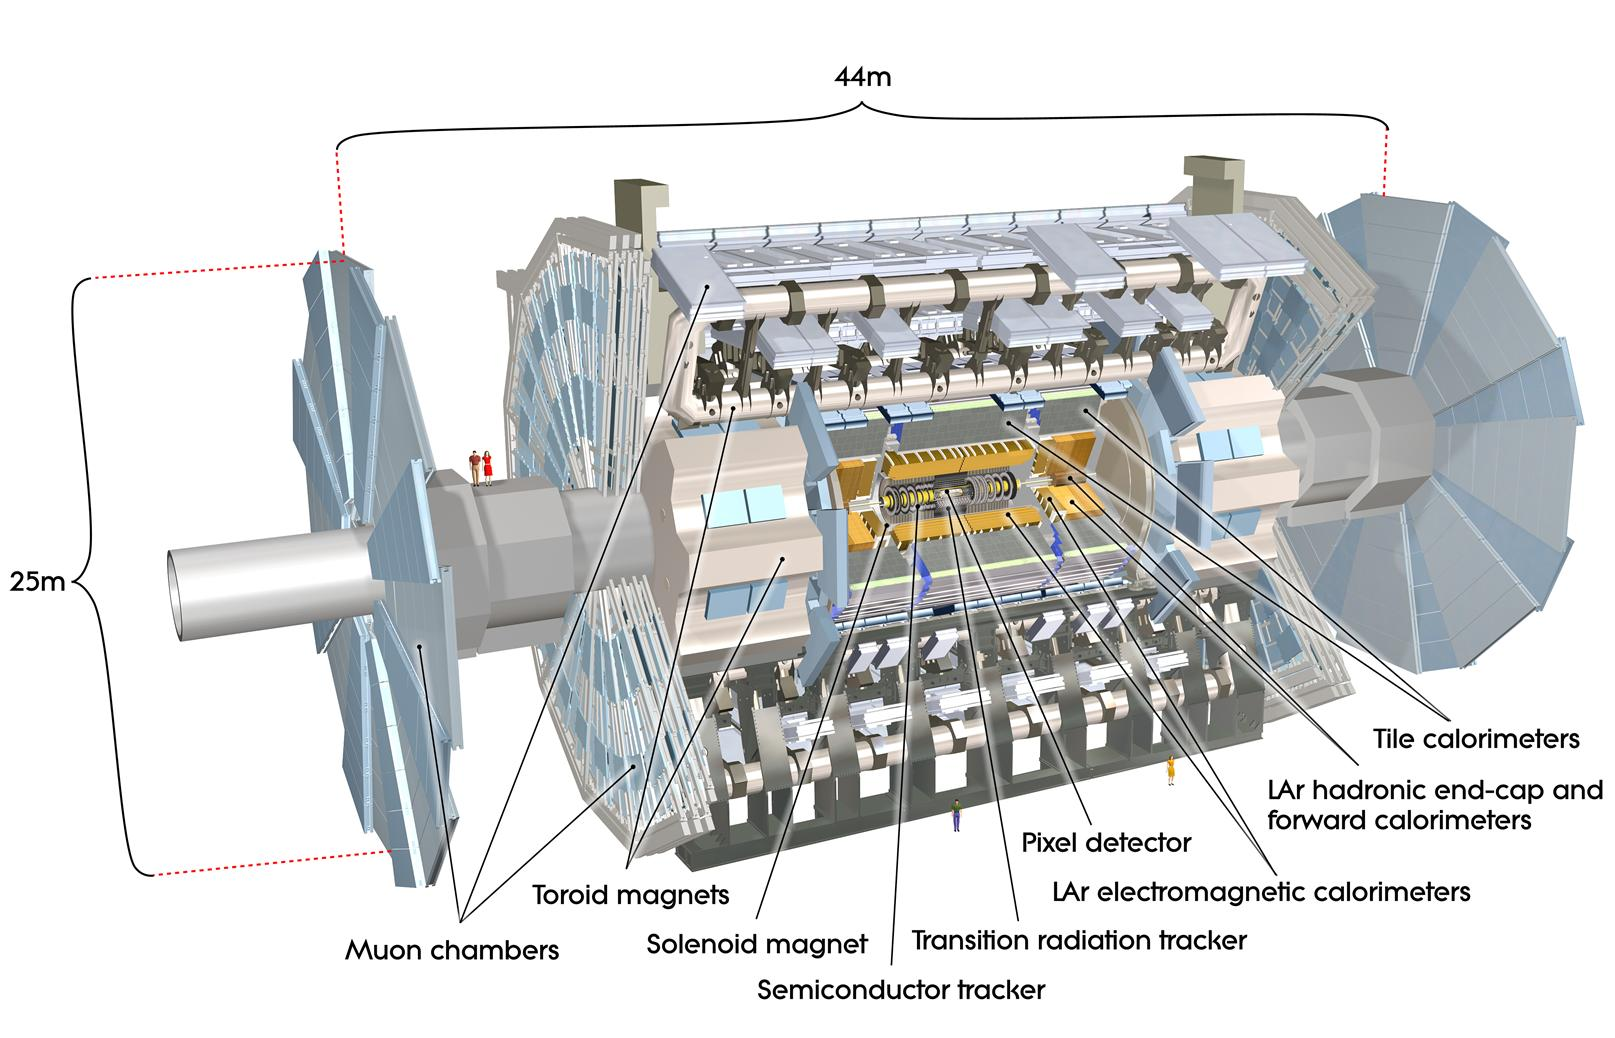
\includegraphics[width=0.9\linewidth]{chapters/2.detector/figs/atlas_detector.jpg}
  \caption{
    A 3D model of the entire \ATLAS detector. 
    Cutouts through the detector }
  \label{fig:atlas_detector}
\end{figure}
%


\subsection{The Inner Detector}\label{sec:atlas_id}

The inner-detector system (ID) provides high-resolution charged particle trajectory tracking in the range $|\eta| < 2.5$.
The ID is immersed in a \SI{2}{\tesla} axial magnetic field, produced by a superconducting solenoidal magnet, which enables the measurement of particle transverse momentum and charge\footnote{Reconstructed charged particles are assumed to have a charge of $\pm 1$.}.
% Momentum resolution is sufficient to identify the charge sign of particles up to the highest energies expected at LHC.
After \runthree, the ID will be replaced by the ITk \cite{ATLAS-TDR-30,ATLAS-TDR-25}.

The inner detector is made up of several sub-systems, shown in \cref{fig:atlas_id_run1,fig:atlas_id_run2}.
The high-granularity silicon pixel detector covers the vertex region and typically provides four spacepoint measurements per track.
It is followed by the silicon microstrip tracker (SCT), which usually provides a further four spacepoint measurements per track.
These silicon detectors are complemented by the Transition Radiation Tracker (TRT),
which enables radially extended track reconstruction up to \(|\eta| = 2.0\). 

\begin{figure}[!htpb]
  \centering
  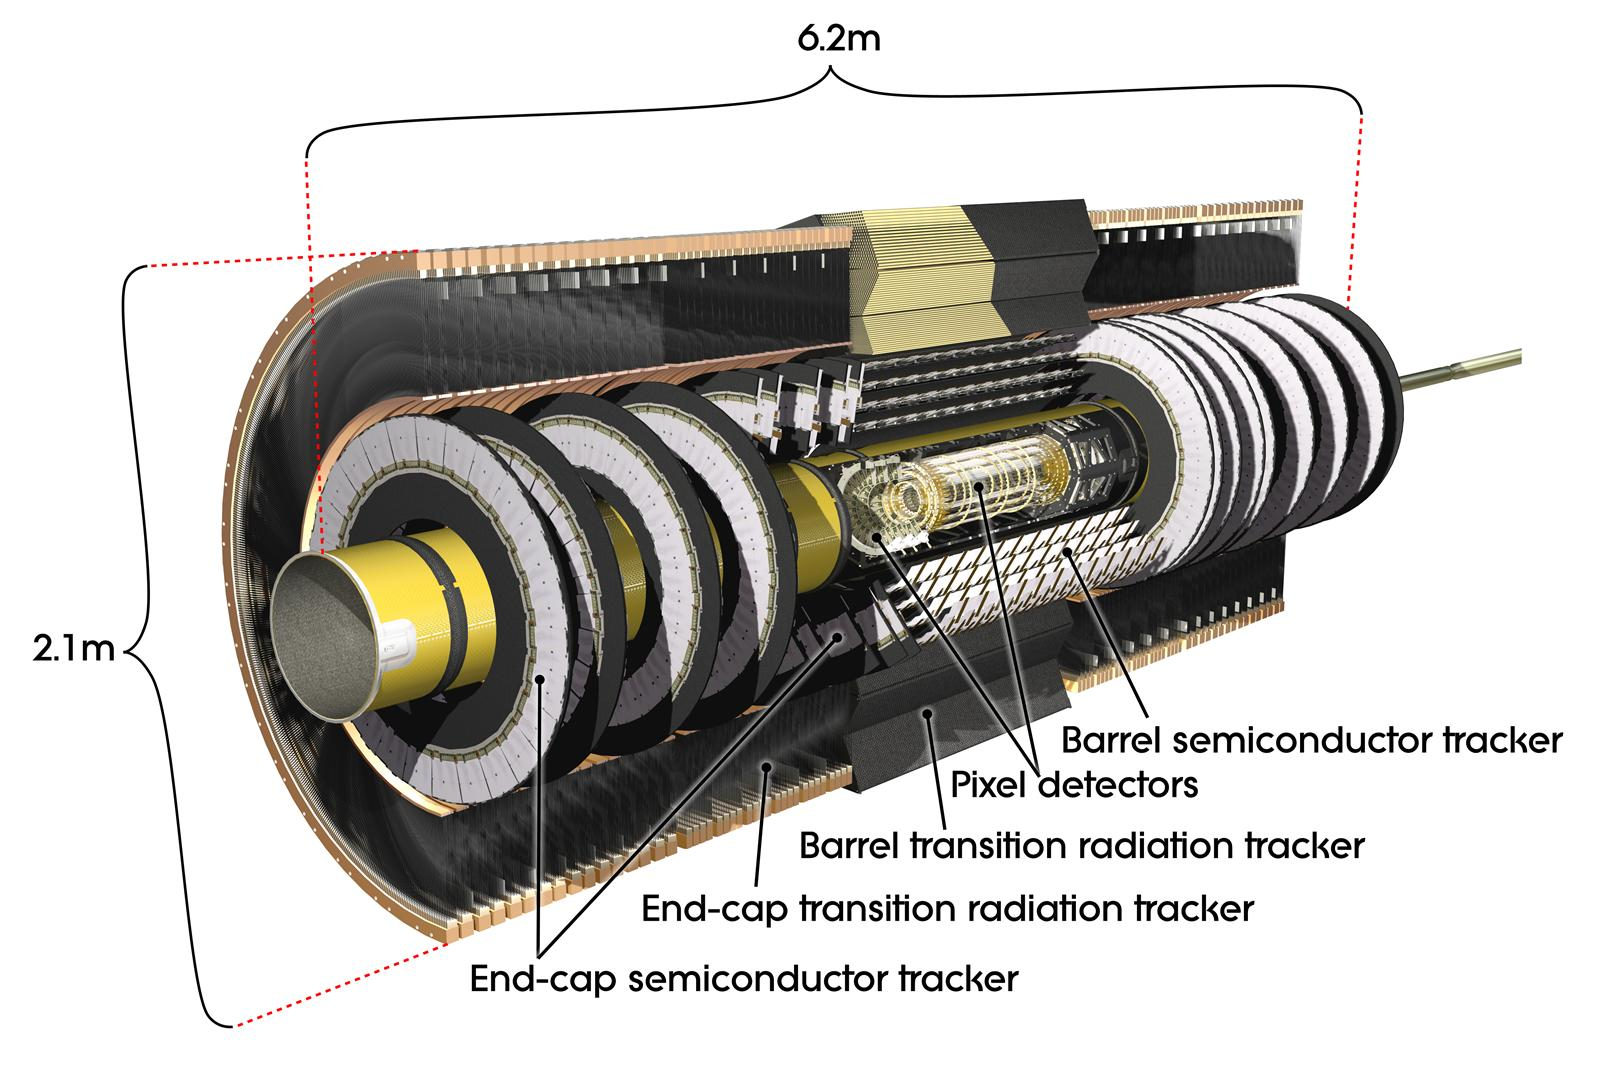
\includegraphics[width=0.75\linewidth]{chapters/2.detector/figs/atlas_id.jpg}
  \caption{A 3D model of the \ATLAS ID showing the barrel layers and end-cap disks.}
  \label{fig:atlas_id_run1}
\end{figure}
%
\begin{figure}[!htpb]
  \centering
  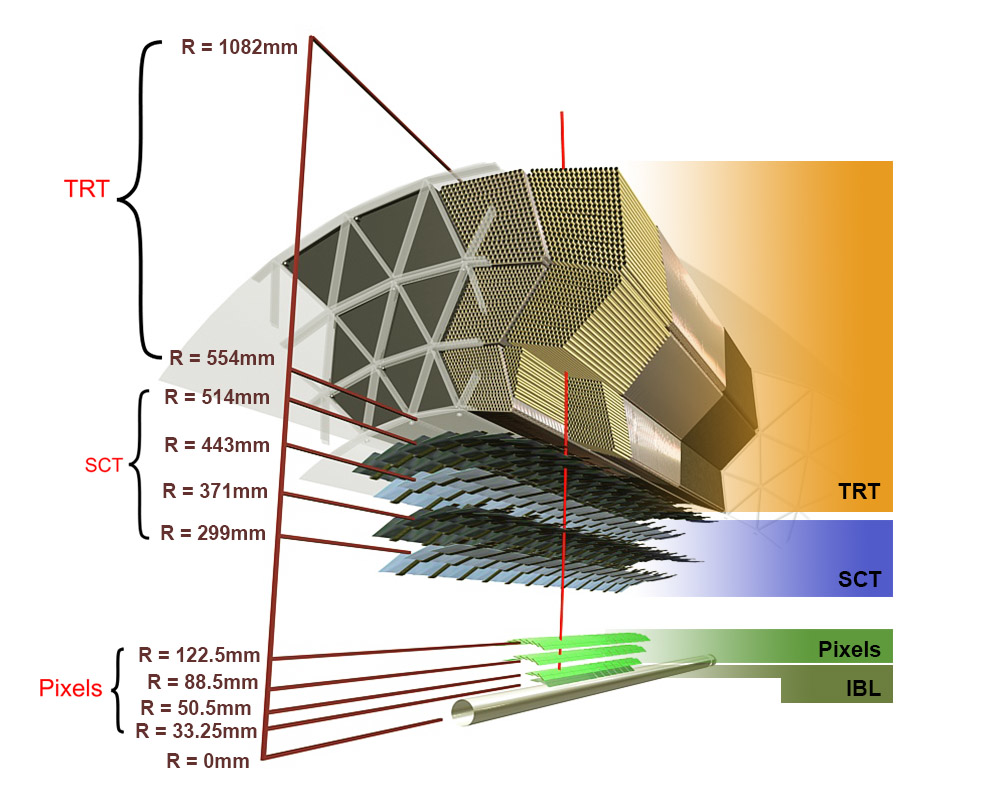
\includegraphics[width=0.75\linewidth]{chapters/2.detector/figs/atlas_id_xs.png}
  \caption{A cross-sectional view of the \ATLAS ID, with the radii of the different barrel layers shown.}
  \label{fig:atlas_id_run2}
\end{figure}
%

\subsubsection{Pixel Detector}
The silicon pixel detector is comprised of four cylindrical barrels at increasing radii from the beamline, and four disks on each side.
The innermost barrel layer is the insertable B-layer (IBL), which was installed before \runtwo \cite{ATLAS-TDR-19,PIX-2018-001} and lies just \SI{33}{\milli\meter} from the beam axis.
%Radiation-hard electronics are used to read out the 140 million channels.
The specification of the pixel detector determines the impact parameter resolution and the ability to reconstruct primary and secondary vertices.
The detector is required to have a high granularity (i.e. resolution) to maintain the low occupancy required to resolve nearby particles. %(high sparsity to resolve different tracks).
Individual pixels are \SI{50}{\micro\meter} in the transverse direction $R\phi$ and \SI{400}{\micro\meter} in the longitudinal $z$ direction (\SI{250}{\micro\meter} for the IBL).
Cluster positions have a resolution of approximately \SI{10}{\micro\meter} in $R\phi$ and \SI{100}{\micro\meter} in $z$.

%giving a resolution of 10 µm in the transverse direction and 115 µm in the longitudinal direction in the barrel region.
%For the IBL, pixels are \SI{50}{\micro\meter} in the $R\phi$ direction and \SI{250}{\micro\meter} in the $z$ direction, giving a cluster resolution of 10 µm in the transverse direction and 115 µm in the longitudinal direction in the barrel region.
%%Pixel clusters and provide an Xlocal resolution of about 10 µm, depending on the particle incident angle

\begin{figure}[!htpb]
  \centering
  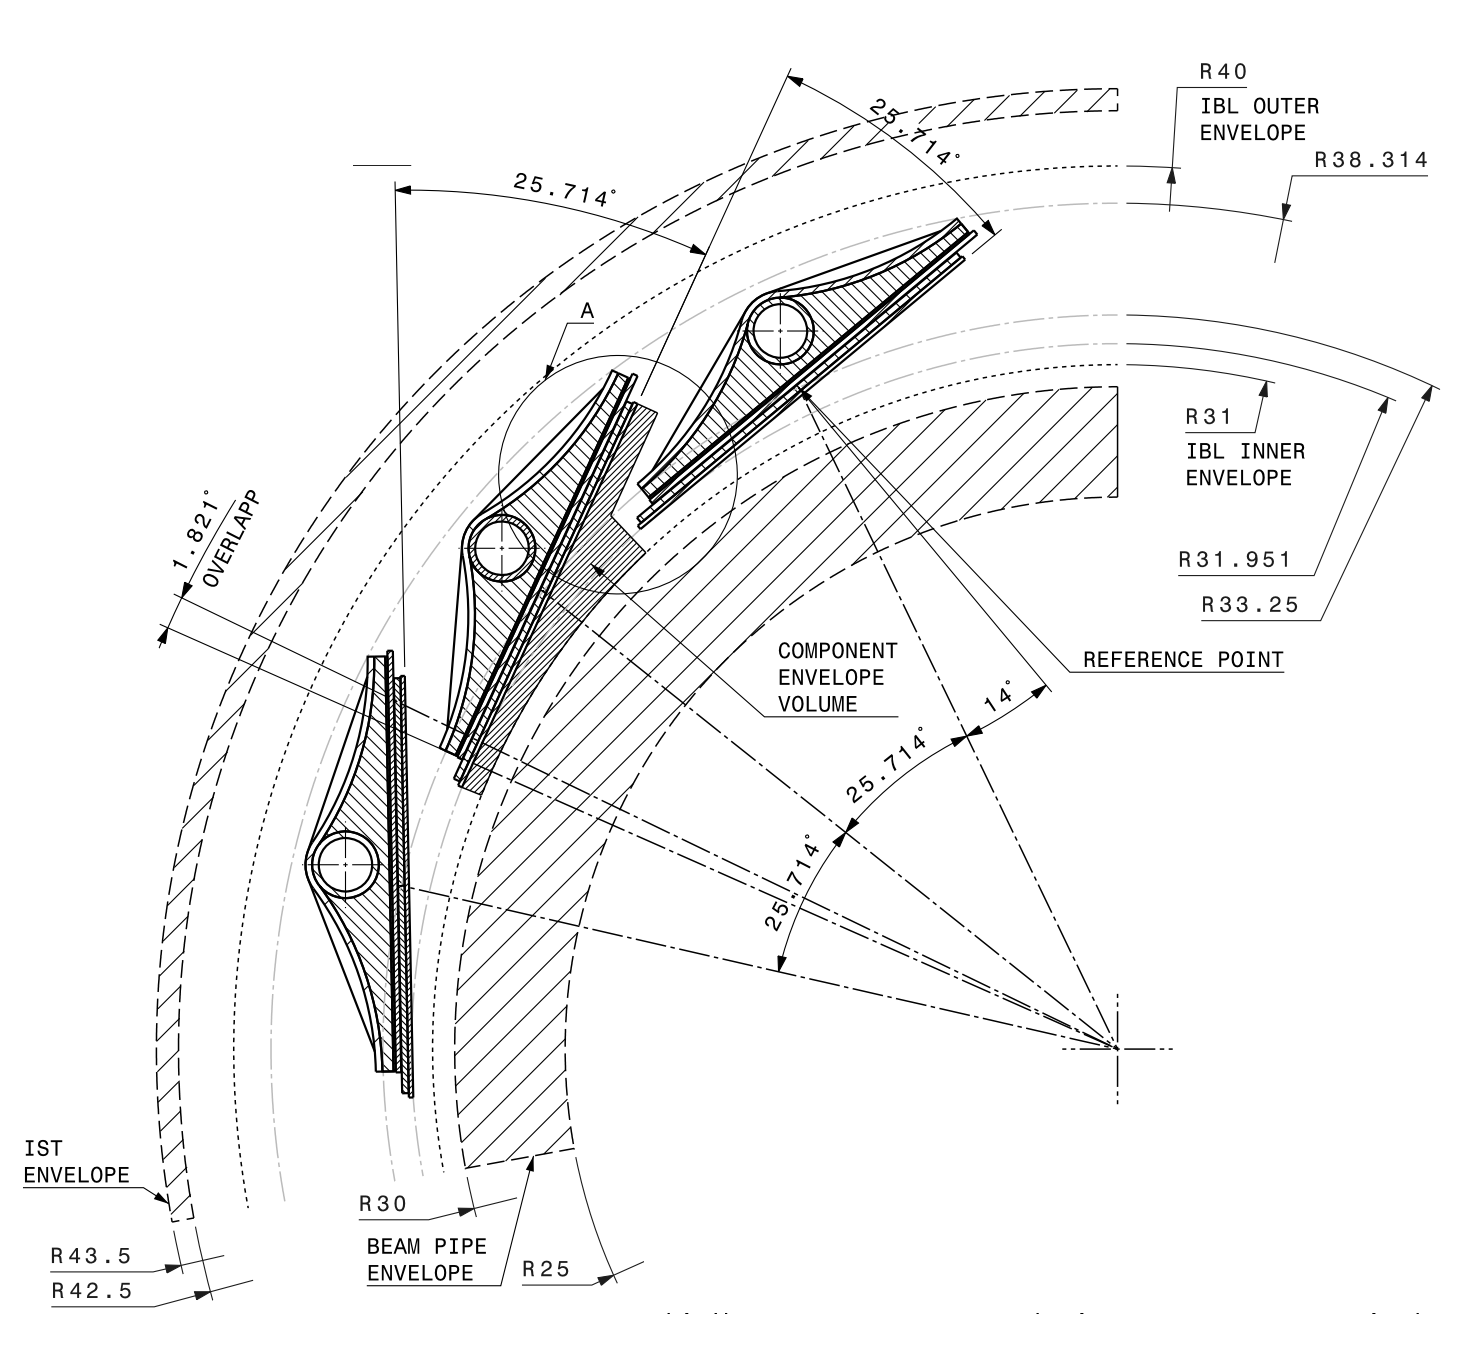
\includegraphics[width=0.6\linewidth]{chapters/2.detector/figs/atlas_ibl.png}
  \caption{A cross-sectional view of the \ATLAS IBL.}
  \label{fig:atlas_ibl}
\end{figure}

\subsubsection{Semi-Conductor Tracker (SCT)}
The SCT is made up of four concentric barrel layers in the central region, and nine disks in each end-cap.
Each layer is itself made of a pair of silicon microstrip layers, with a small stereo angle (\SI{20}{\milli\radian}) between the two layers enabling the $z$\nobreakdash-coordinate measurement from a pair of strip measurements.
The SCT typically provides four precision spacepoint measurements (eight strip measurements) per track in the barrel region.
These have intrinsic uncertainties of \SI{17}{\micro\meter} in the transverse direction $R\phi$, and \SI{580}{\micro\meter} in the longitudinal direction $z$.
The measurements provide a key contribution to the measurement of charged particle momentum and impact parameter, along with vertex position.
%The high granularity enables good pattern recognition
Charge-particle tracks can be distinguished if separated by more than $\sim \SI{200}{\micro\meter}$.
Hits are registered as binary signals if the pulse height in a channel exceeds a certain threshold.


\subsubsection{Transition Radiation Tracker (TRT)}
The TRT is a straw-tube tracker which complements the higher-resolution silicon-based tracks by offering a larger number of hits per track (typically around 30) and a long lever arm, which aids the accurate measurement of particle momentum. 
It is made up of approximately \num{300000} drift tubes with a diameter of \SI{4}{\milli\meter} which are filled with xenon gas.
The walls of each tube are electrically charged, and a thin conducting wire runs along the center.
When a charged particle traverses a tube, it ionises the xenon and the resulting liberated electrons drift along the electric field to the wire, where an associated charge is registered.
In the barrel the straws run parallel to the \axis{z} and therefore the TRT only provides tracking information in $R\phi$. Straws are arranged radially in the end-caps. The resulting two-dimensional spacepoints have a resolution of approximately \SI{120}{\micro\meter}.
The spaces between the straws are filled with a polymer which leads to the emission of transition radiation, aiding electron identification.

%It allows the ID to reconstruct $V_0$s which are especially interesting in CP-violating $B$ decays.
%Electron identification capability is added by employing xenon gas to detect transition-radiation photons created in a radiator between the straws. In addition it provides additional discrimination between electrons and hadrons
% provides electron identification information based on the fraction of hits (typically 30 in total) above a higher energy-deposit threshold corresponding to transition radiation.
%may be emitted by highly relativistic charged particles as they traverse a material boundary. This effect depends on the relativistic factor γ = E/m and is strongest for electrons, 
%means it can be used for particle identification (section 6). Typical photon energies are 5–30 keV. These soft X-rays can be absorbed by Xe atoms, depositing additional energy in the gas and leading to significantly higher readout signals. Suc

%Within the radial space available, the straw spacing has been optimised for tracking at the expense of electron identification, which would be improved by a greater path length through the radiator material and fewer active straws. 


% TR is a form of electromagnetic radiation emitted when a charged particle passes through inhomogeneous media, such as a boundary between two different media. The probability that a particle emits radiation is given by it's $\gamma$ (Lorentz) factor (ie particle velocity). Electrons in general have higher Lorentz factors than eg. pions, as they are lighter than pions. In this way, the TRT discriminates between lighter and heavier particles.

\subsection{Calorimeters}\label{sec:calorimeter}

The calorimeter system measures the energy of incident particles over the range $|\eta| < 4.9$.
There are two main sub-systems: the electromagnetic calorimeter (ECal), which focuses on the measurement of electrons and photons, and the hadronic calorimeter (HCal), which measures the energy of hadrons.
Upon entering the calorimeter, incident particles will interact with the detector material to produce a shower of secondary particles with reduced energies. 
The charge deposited in this process is measured to reconstruct the energy of the initial incident particle.
The two calorimeter sub-systems must must provide strong containment of showering particles to prevent punch-through of EM and non-muon particles to the HCal and muon system respectively.

%the fine granularity of the EM calorimeter is ideally suited for precision measurements of electrons and photons. The coarser granularity of the rest of the calorimeter is sufficient to satisfy the physics requirements for jet reconstruction and $E_T^{\textrm{miss}}$ measurements.     

%A narrow transverse profile is characteristic of an electromagnetic cascade. Hadrons passing through matter also initiate cascades through inelastic hadron-nuclei interactions. The shower produces secondary hadrons and leptons and has a comparatively wide transverse profile. 

%Nuclear interaction length is the mean distance travelled by a hadronic particle before undergoing an inelastic nuclear interaction.
%The nuclear interaction length is about an order of magnitude greater than the radiation length of the material. Therefore, like most general purpose experiments, ATLAS uses two different calorimetry systems to measure electrons and photons (the ECal) and hadrons (the HCal). 

%
\begin{figure}[!htpb]
  \centering
  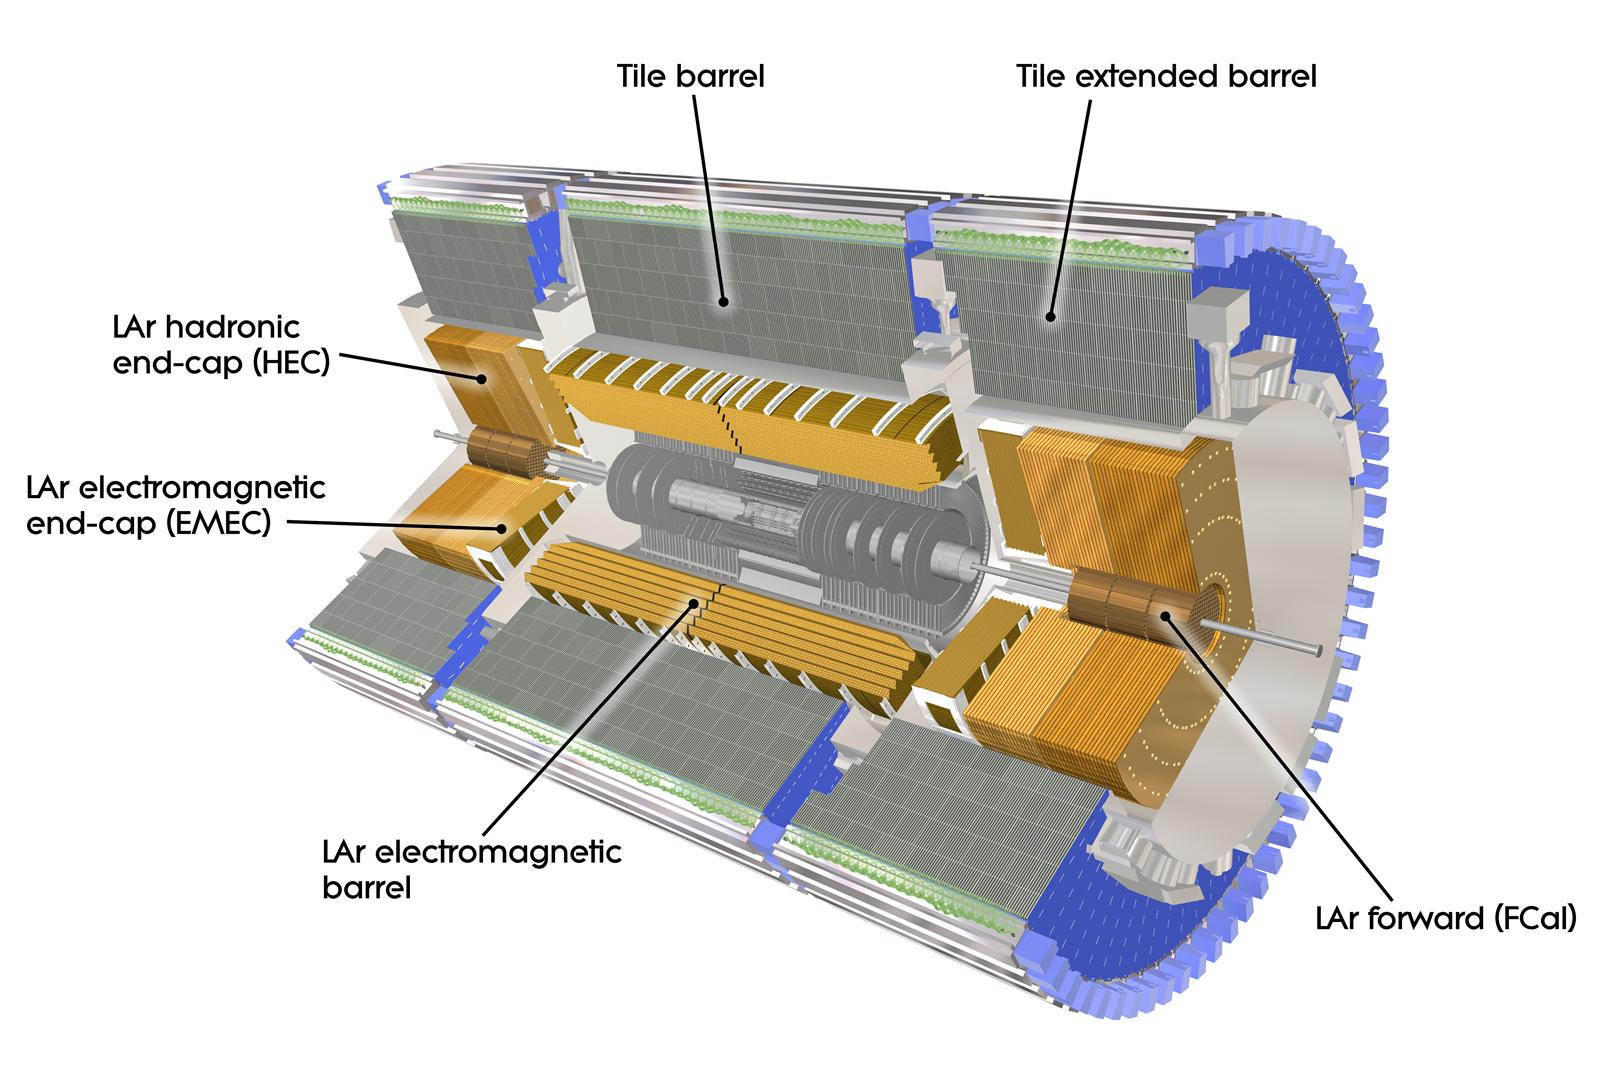
\includegraphics[width=0.8\linewidth]{chapters/2.detector/figs/atlas_calos.jpg}
  \caption{The \ATLAS calorimeters. The ECal (orange) and HCal (grey, brown).}
  \label{fig:atlas_calos}
\end{figure}
%


\subsubsection{Liquid Argon (LAr) Electromagnetic Calorimeter}
The more granular lead/liquid-argon ECal covers the region $|\eta|< 3.2$ and is split into barrel (covering $|\eta| < 1.475$) and end-cap (covering $1.375 < |\eta| < 3.2$) regions.
EM calorimetry works by encouraging electrons and photons to interact with electrically charged particles in detector material via bremsstrahlung ($e \rightarrow e\gamma$) and pair production ($\gamma \rightarrow e^+ e^- $).
The EM calorimeter uses lead absorber plates to initiate EM showers, resulting in secondary particles which ionise the surrounding liquid argon.
The charge is collected on copper electrodes and read out.
The accordion geometry of the ECal allows for a full coverage in $\phi$ without any azimuthal cracks. 

%it initiates an electromagnetic cascade,
%The fine granularity of the EM calorimeter
%Additionally, multiple samplings of the shower are used to resolve its pointing vector.

\subsubsection{Hadronic Tile Calorimeter}
In the central barrel region with $|\eta| < 1.7$, the HCal uses a tile calorimeter with steel as an absorbing material, and scintillating tiles as the active material.
Two copper/liquid-argon calorimeter end-caps are also used.
Incident hadrons interact via the strong and electromagnetic forces with the absorber material, mainly loosing energy due to multiple inelastic nuclear collisions.
The active material captures the resulting electrons and photons to measure the energy of the incident hadron.

%Hadrons are relatively massive and cannot radiate much of their energy through bremsstrahlung, and they lose their energy mainly through multiple nuclear collisions.  Hadrons passing through matter also initiate cascades through inelastic hadron-nuclei interactions.

%The tile calorimeter is placed directly outside the EM calorimeter envelope.o 
%The barrel covers the region -1.0<η<1.0, and the extended barrels cover the region 0.8<|η|<1.7.

%LAr hadronic end-cap calorimeter (HEC). Located directly behind (in $z$) the end-cap electromagnetic calorimeter and sharing the same LAr cryostats. The high level of radiation in the forward regions would cause severe damage to plastic scintillators. In the end-caps, parallel copper plates are submerged in liquid argon, which is preferred as the active medium because of its inherent radiation hardness.


\subsection{Muon Spectrometer}\label{sec:muon_spectrometer}
Due to their higher mass, muons easily pass unimpeded through the ID and calorimeters and therefore require specialised detectors for their measurement.
% higher mass means brem is less effective at slowing them down. though
The Muon Spectrometer (MS) is made up of dedicated tracking and triggering hardware.
The precision tracking system uses three layers of monitored drift tubes with a barrel region covering $|\eta| < 1.2$ and end-caps covering $1 < |\eta| < 2.7$. The inner layers of the end-caps use cathode strip chambers to better cope with the high occupancy in the forward region.
Precision tracking resolution is approximately \SI{50}{\micro\meter}.
The trigger system is comprised of resistive plate chambers in the barrel region covering $|\eta| < 1.0$ and thin gap chambers in the end-cap regions covering $1 < |\eta| < 2.4$.
A set of three toroidal magnets, each made up of eight coils, is used in each of the barrel and end-caps to deflect the muons as the pass through the MS, allowing their momentum and charge to be measured from the direction and magnitude of curvature.
The toroidal magnets generate a field which is largely orthogonal to the muon trajectories which allows for maximum deflection.
%
\begin{figure}[!htpb]
  \centering
  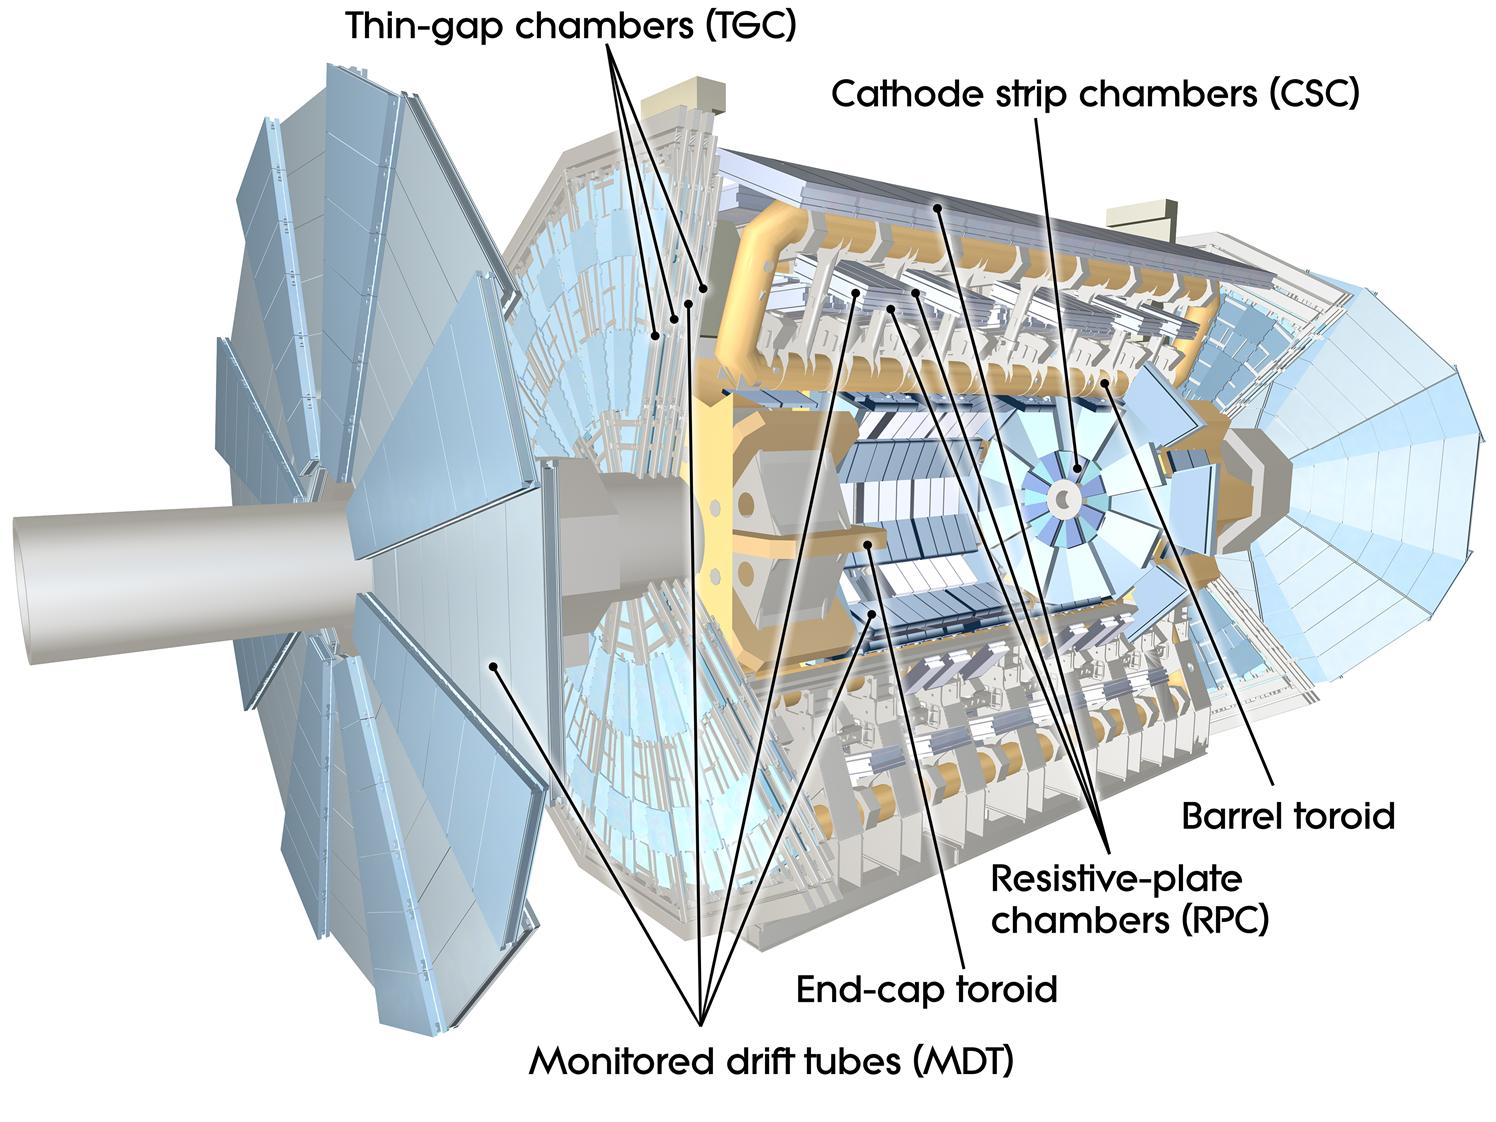
\includegraphics[width=0.7\linewidth]{chapters/2.detector/figs/atlas_muon_system.jpg}
  \caption{The \ATLAS muon spectrometer.}
  \label{fig:atlas_muon_system}
\end{figure}
%


\subsection{The Trigger}\label{sec:trigger}
The \SI{2.5}{\nano\second} bunch spacing used over the course of \runtwo corresponds to a bunch-crossing or event rate of \SI{40}{\mega\hertz} (see \cref{tab:lhc_runs}).
If the full information for the detector was written out for each event, this would correspond to the generation of \SI{60}{\tera\byte} of data each second.
This is more than can be feasibly processed and stored, requiring the use of a trigger system which quickly makes a decision about whether or not an event is potentially interesting and should be kept for further analysis.
The trigger system is comprised of two levels which search for signs of electrons, muons photons, taus and jets, as well as events with high total or missing transverse energy.
The hardware-based Level-1 (L1) trigger uses coarse information from the calorimeters and MS to accept events at a rate of \SI{100}{\kilo\hertz} within \SI{2.5}{\micro\second} of the event.
After the L1 trigger, the software-based High Level Trigger (HLT) makes use of \num{40000} CPU cores to make a final selection on surviving events within a few hundred milliseconds. 
The final event read-out rate is approximately \SI{1.2}{\kilo\hertz}, corresponding\SI{1.2}{\giga\byte\per\second} of permenant data storage.
More information is provided in \cite{TRIG-2016-01}.
%Regions of Interest (ROIs) from the L1 trigger are used.

%The L1 trigger searches for high transverse-momentum muons, electrons, photons, jets, and $\tau$-leptons decaying into hadrons, as well as large missing and total transverse energy. Its selection is based on information from a subset of detectors. High transverse-momentum muons are identified using trigger chambers in the barrel and end-cap regions of the spectrometer. Calorimeter selections are based on reduced-granularity information from all the calorimeters. Results from the L1 muon and calorimeter triggers are processed by the central trigger processor, which implements combinations of different trigger selections. In each event, the L1 trigger also defines one or more Regions-of-Interest (RoI’s), i.e. the geographical coordinates in $\eta$ and $\phi$, of those regions within the detector where its selection process has identified interesting features. The RoI data include information on the type of feature identified and the criteria passed, e.g. a threshold. This information is subsequently used by the high-level trigger.

%The L2 selection is seeded by the RoI information provided by the L1 trigger. L2 selections use, at full granularity and precision, all the available detector data within the RoI’s (approximately 2\% of the total event data). The L2 menus are designed to reduce the trigger rate to approximately 3.5 kHz, with an event processing time of about 40 ms, averaged over all events. The final stage of the event selection is carried out by the event filter, which reduces the event rate to roughly 200 Hz. Its selections are implemented using offline analysis procedures within an average event processing time of the order of four seconds.










\section{Reconstructed Physics Objects}\label{sec:physics-objects}

Event reconstruction is the process of analysing the raw signals from the detector to determine the type and properties of particles present in an event. 
The reconstructed event provides information about the underlying physics process that led to the observable final state. 
Events passing the trigger selection (described in \cref{sec:trigger}) undergo full offline reconstruction, which makes use of the full information from the detector.
Reconstruction and analysis of events relies on the extensive \ATLAS software stack, see \rcite{ATL-SOFT-PUB-2021-001} for more information.

Several different reconstructed objects are used for physics analyses.
Objects relevant to the analyses described in this thesis are described below.



\subsection{Tracks}\label{sec:track_reco}
The trajectories of charged particles are reconstructed as tracks from the energy depositions (called \textit{hits}) left by the particles as they traverse the sensitive elements of the inner detector.
Tracks are used for a variety of downstream applications, including vertexing and jet tagging.
A comprehensive introduction to ATLAS tracking is available in \cite{Cornelissen:2007vba}, while specific optimisations for dense environments are detailed in \cite{ATL-PHYS-PUB-2015-006, PERF-2015-08}.
An overview of track reconstruction is given below.

%Tracking is useful for: impact parameter measurements, vertexing for heavy-flavour and $\tau$ tagging.

\subsubsection{Space-point Formation (Clustering)}
When a charged particle traverses a pixel layer, charge is typically collected in more than one pixel. 
This is due to the incident angle of the particles with respect to the sensor, and also the drift of electrons between sensors caused by the magnetic field.
Clusters (also called \textit{hits} or \text{space-points}) are formed by clustering neighbouring pixel cells and estimating locations of space-points using the shape and energy distribution of the clusters.

\subsubsection{Track Finding}
Space-points are used to build track seeds. These are groups of three hits which are geometrically compatible with being part of a track segment.
A combinatorial Kalman filter (KF) is used to build track candidates by extending track seeds.
The filter can create multiple track candidates per seed, with bifurcations along the track occurring when more than one compatible space-point exists on a given layer.
In this way, the KF creates an excessive number of \textit{track candidates}, which are only required to satisfy basic quality requirements. 
Track candidates are allowed to reuse or \textit{share} hits freely (a single hit may be used by multiple track candidates).
Typically, the presense of shared hits is a predictor of a bad track due to the high granularity of the ATLAS tracking detectors.
At this stage, there is a large number of incorrect hits assigned to otherwise good tracks, and additionally large number of \textit{fake} tracks, which are comprised of a majority of wrong hits and do not correspond to the trajectory of any one physical particle (fake tracks are defined as those where the majority of associated hits do not originate from one single truth particle).\todo{TMP def}
The low quality of tracks at this stage necessitates an ambiguity solving step, in which candidates are cleaned, and the highest quality track are selected.

\subsubsection{Ambiguity Solving}
Ambiguity solving was introduced as part of the ATLAS New Tracking effort (NEWT) \cite{Cornelissen:2007vba}, and is intended to improve track reconstruction performance in challenging dense environments.
In the ambiguity solver, track candidates are processed individually in descending order of a track score. The track score quantifies the likelihood of the track corresponding to the trajectory of a real particle. Scoring uses a number of signals, including the number and positions of hits (preferring hits in more precise regions of the detector), the transverse momentum of the track and the track fit quality. The track fit quality describes the quality of the track as the $\chi^2$ divided by the number degrees of freedom on the track. A preference for high transverse momentum tracks promotes the successful reconstruction of the more physically interesting energetic particles, and suppresses the large number of wrong hits assigned to low momentum tracks.

During the processing of a given highest-scoring track candidate, the track is cleaned (whereby problematic hits are removed), and, if the cleaning is successful, a full resolution fit is performed. If the track has reached this stage without rejection by passing various quality regiments, it is re-scored and returned to the list of track candidates. If the same track is then processed again without requiring modification, it is added to the final track collection. Track candidates that fall beyond a certain quality cut are rejected. This cut does allow the possibility of a track passing through the ambiguity solver with a small number of shared hits.\todo{list shared hit cut }

\subsubsection{Neural Network Cluster Splitting}
As part of track cleaning, shared hits are classified by a Neural Network (NN) to determine if they are compatible with the characteristic features of a merged cluster \cite{2014arXiv1406.7690A, ATL-PHYS-PUB-2015-006}.
A merged cluster is one which has originated from more than one incident particle.
The corresponding reconstructed cluster is made up of a combination of energy deposits from more than one particle, which have become merged due to the closeness of the associated particles and the limited resolution of the detector.
While in general this event is rare, it is common for clusters to become merged in dense environments, as discussed in \cref{sec:b_had_reco}.
If the cluster is predicted to be merged it is labelled as being freely shareable, or \textit{split}.
Hits classified as split by the cluster splitting NN are allowed to be shared freely.
Hits not compatible with the merged hypothesis can still be shared by a limited number of tracks, but come with a penalty for the track which may hinder its acceptance into the final track collection.
%
\begin{figure}[ht]
    \centering
    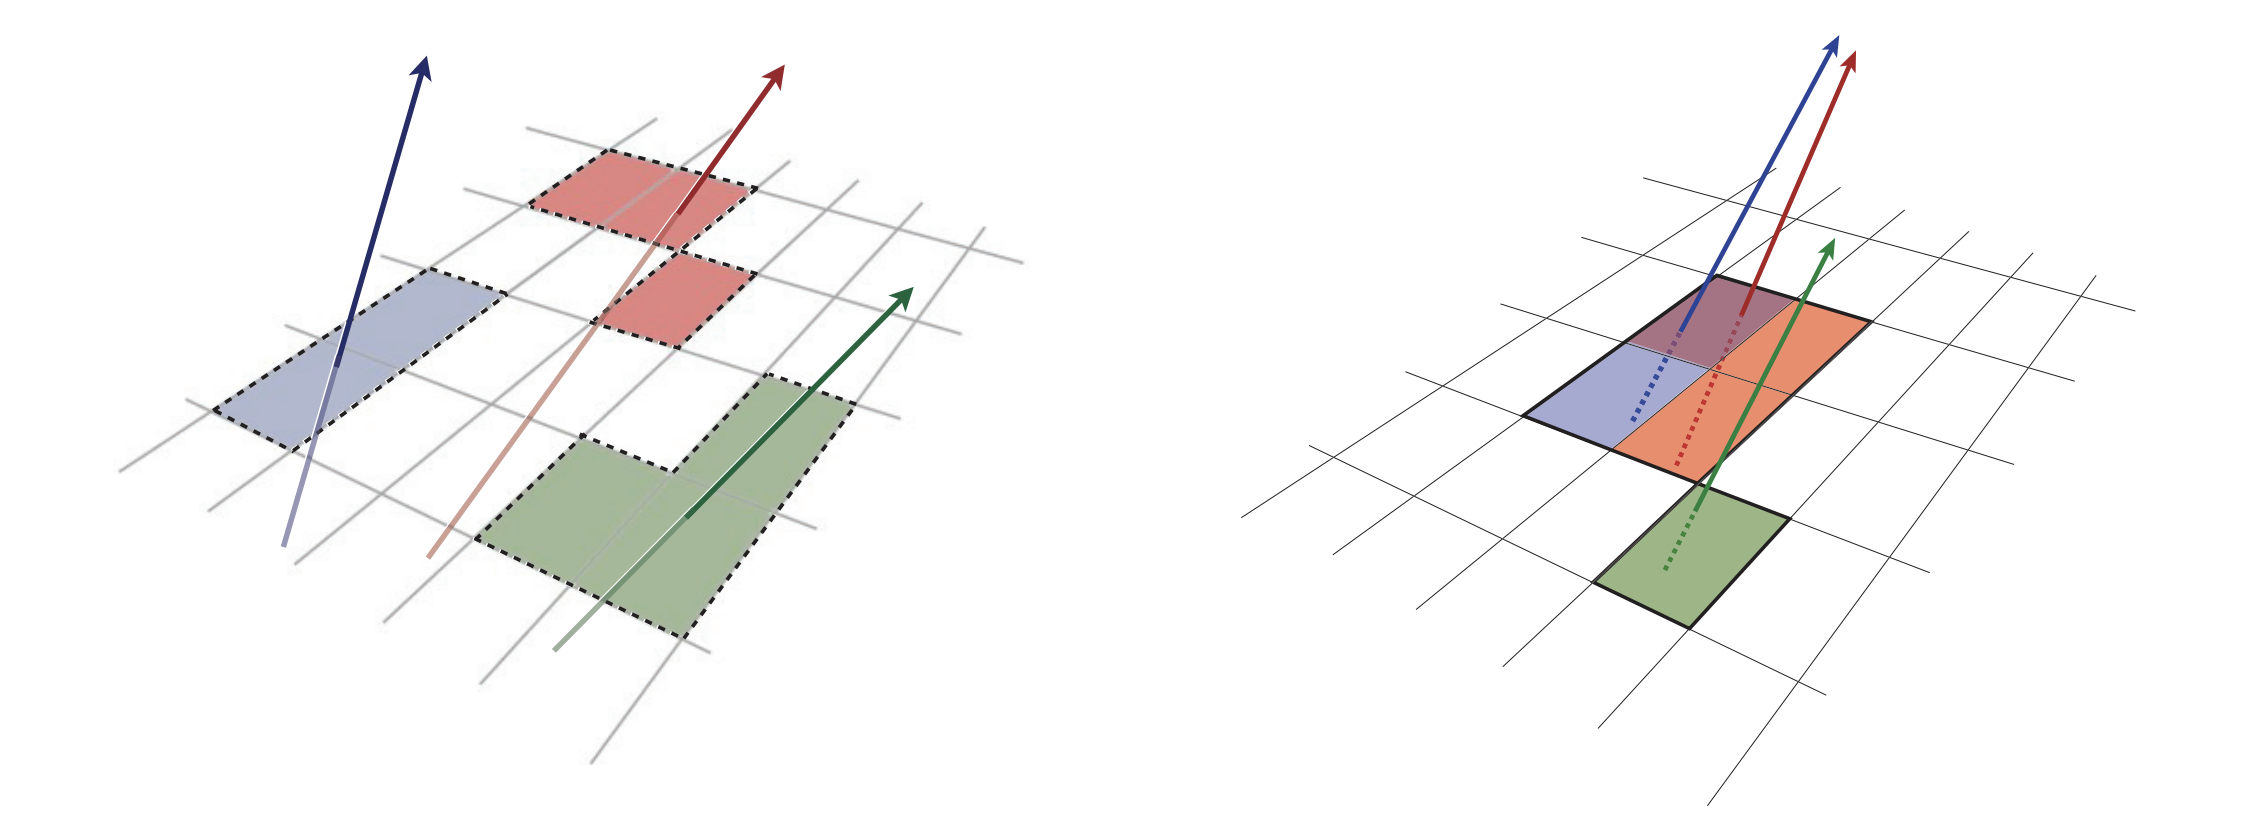
\includegraphics[width=0.8\textwidth]{chapters/2.detector/figs/merged-cluster.png}
    \caption{
      Particles (left) which have enough separation will leave charge depositions which are resolved into separate clusters.
      Sufficiently close particles (right) can lead to merged clusters.
      Their combined energy deposits are reconstructed as a single merged cluster.}
    \label{fig:resolved/merged clusters}
\end{figure}
%


\subsection{Vertices}\label{sec:vertex_reco}
Groups of reconstructed tracks can be examined to determine whether the particles originated from a common spatial point of origin.
This occurs when a particle decays or radiates.

\subsubsection{Primary Vertices}
Each proton-proton interaction happens at a \textit{primary vertex} (PV).
Primary vertices are iteratively reconstructed using tracks.
The \textit{hard scatter vertex} of an event is chosen as the primary vertex whose associated tracks have the largest sum of transverse momentum squared, $\Sigma\pt^2$.

\subsubsection{Secondary Vertices}
Secondary vertices occur when a particle radiates or decays at a sufficient distance from the primary vertex to be resolved.
See \cref{sec:b_decay_topology}.
Two widely used secondary vertexing tools are used within \ATLAS.
Each attempts to reconstruct vertices given the tracks associated with a jet (see \cref{sec:jet_reco}).
The first, SV1 by design attempts to find a single inclusive vertex per jet.
The second, JetFitter


\subsection{Jets}\label{sec:jet_reco}
Jets are the reconstructed object corresponding to a spray of collimated stable particles which results from a decay chain.
Jets are built by clustering constituent objects (e.g. tracks or calorimeter clusters) using a jet finding algorithm, for example the anti-$k_T$ algorithm \cite{Cacciari:2008gp}.

\subsubsection{Particle Flow Jets}
Jets are reconstructed from particle-flow objects \cite{PERF-2015-09} using the anti-$k_T$ algorithm with a radius parameter of $0.4$.
The jet energy scale is calibrated according to \rcite{PERF-2016-04}.
Jets are also required not to overlap with a generator-level electron or muon from \Wboson boson decays.
All jets are required to have a pseudorapidity $|\eta| < 2.5$ and $\pt > \SI{20}{\GeV}$. 
Additionally, a standard selection using the Jet Vertex Tagger (JVT) algorithm at the tight working point is applied to jets with $\pt < \SI{60}{\GeV}$ and $|\eta| < 2.4$ in order to suppress pile-up contamination \cite{ATLAS-CONF-2014-018}.
Tracks are associated to jets using a \DeltaR association cone, the width of which decreases as a function of jet \pt, with a maximum cone size of $\DeltaR \approx 0.45$ for jets with $\pt = \SI{20}{\GeV}$ and minimum cone size of $\DeltaR \approx 0.25$ for jets with $\pt > \SI{200}{\GeV}$. 
If a track is within the association cones of more than one jet, it is assigned to the jet which has a smaller $\DeltaR(\text{track}, \text{jet})$.

Jet flavour labels are assigned according to the presence of a truth hadron within ${\DeltaR(\text{hadron},\text{jet})<0.3}$ of the jet axis. If a \bhadron is found the jet is labelled a \bjet. In the absence of a \bhadron, if a \chadron is found the jet is called a \cjet.
If no \borchadrons are found, but a $\tau$ is found in the jet, it is labelled as a $\tau$-jet, else it is labelled as a \ljet.

\subsubsection{Track Jets}
???



\subsection{Leptons}\label{sec:lepton_reco}

Electrons and muons are stable leptons and leave characteristic signatures that are picked up in the ECal and MS respectively.
The reconstruction of both types of of stable lepton is briefly outlined below.

\subsubsection{Electrons}
Electrons candidates are reconstructed by matching PV-compatible inner detector tracks to calorimeter clusters.
The track-cluster matching criteria takes into account the significant energy loss of the electron due to bremsstrahlung.
If a match is found, a refit of the track is performed using the Gaussian Sum Filter (GSF) \cite{ATLAS-CONF-2012-047}, which better handles trajectory reconstruction in the presence of bremsstrahlung.
Various identification criteria are then applied using a  likelihood-based (LH) method to the candidates to improve purity.
These include requirements on the track quality and cluster matching, the shape of shower in the ECal, leakage into the HCal, and the amount of transition radiation detected in the TRT.
A full description can be obtained in \rcite{ATLAS-CONF-2016-024}.
%
\begin{figure}[!htbp]
  \centering
  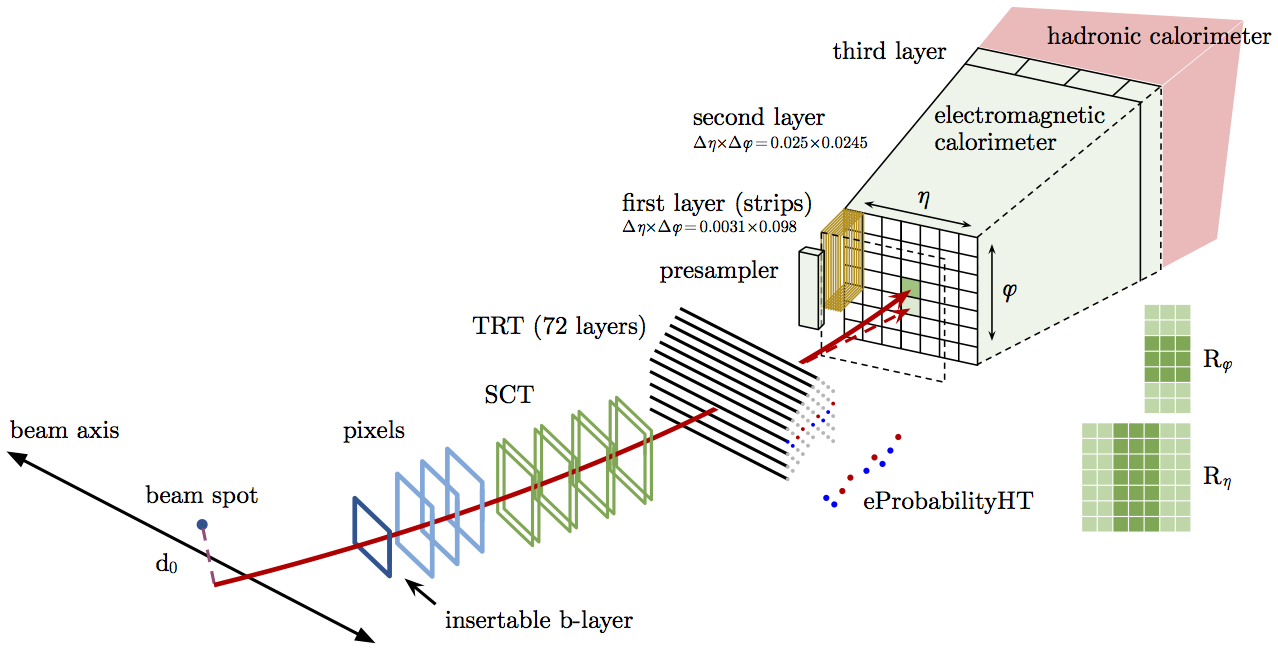
\includegraphics[width=0.8\linewidth]{chapters/2.detector/figs/electron_reco.png}
  \caption{
    A sketch of electron reconstruction using the \ATLAS detector \cite{ATLAS-CONF-2016-024}.
    Electron reconstruction makes use of the entire ID and the calorimeters.
    In particular, discriminating information comes from the TRT and ECal.
  }
  \label{fig:electron_Reco}
\end{figure}
%


\subsubsection{Muons}
Muon reconstruction primarily makes use of the dedicated MS (see \cref{sec:muon_spectrometer}), but also relies on tracks from the ID and the presence of characteristic signatures in the calorimeters.
Muon tracks are reconstructed by connect straight-line track segments, which are identified via a Hough transform, and combined into a approximately parabolic trajectory.
Finally, a global $\chi^2$ fit is performed, taking into account possible interactions between the muon and the detector material.
A reconstructed muon is called \textit{combined} if it completes successful matching to an ID track.
Combined muons undergo a further fit with the combined ID and MS hits, with the energy loss due to the traversal of the calorimeters being taking into account.

